\section{Finding Double-Unlock Bugs}
This section will detail how the abstractions defined previously are integrated into the EBA framework in order to explore the control flow of input programs while generating the product of the control flow and monitor automata in order to detect possible bugs. 

\subsection{Integration into EBA}
In order to implement a new bug checker into EBA, the implementation has to conform to the structure set up by the framework of how these checkers should behave. Furthermore, signatures must be defined for these checkers in order to allow the framework to instantiate these checkers according to user input. This section will describe how this has been accomplished.  

\newpar The EBA framework allows specifying checker signatures whose implementations are executed on a given input source file. Checker signature implementations instantiate a given bug checker for a given bug type and the internal logic of the bug checker is run by the framework. 

\newpar These bug checkers must conform to the existing signatures of EBA in order to allow the framework to instantiate a given bug checker after which an abstract representation of the input source file is passed to the instantiated checker. 

\newpar In order to detect possible bugs in input programs, a control flow graph and an instantiation of the given monitor automata monitoring the control flow are required. The control flow is provided by the EBA framework, while the monitor automata have been defined and implemented as part of my work.   

\newpar A signature for a checker which allows instantiation of monitor automata bug checkers has been defined as part of my work. This signature is then implemented in order to let EBA instantiate the implemented checker. A function, \texttt{check}, is the only requirement for implementing this signature and takes two parameters after which it returns a list of strings for each detected possible bug in the input source file as expected by the EBA framework. These parameters are the abstractions of the input file and each global function defined in this file, both of which are passed to the function by the framework. This mimics the implementation of the existing CTL checkers in EBA and allows for easy integration into the framework. 

\newpar The aforementioned signature is implemented as a module, \texttt{Make}, which is used by EBA in order to run automata bug checkers conforming to an automata signature. Specifying a signature which all automata-based checkers must conform to ensures that the automata expose the required state and transition functions for them to run. This \texttt{Make} module expects an implementation of this \texttt{AutomataSpec} signature. 

\newpar The \texttt{check} of the \texttt{Make} module explores the CFG provided by the EBA framework of the given file and applies the transition of the monitor automata using the effects of statements, which are represented as nodes in the CFG. The tree is then explored further until the end of each path in the tree is explored, resulting in a set of monitor automata states, which can then be explored in order to determine if any automata have reached accepting states. If such a state is present, a possible bug has been discovered. 

\newpar Nodes in the CFG structure provided by EBA be one of four different types, each representing the input statement. Nodes representing if-statements in the source input result are \textit{If}-nodes in the tree, containing two branches. If an If-node is discovered, the two branches from that node are explored and the union of the resulting states is found. Nodes representing the end of a branch are \textit{Nil}-nodes in the tree. Nodes representing assumptions made after if-statements are either true or false are \textit{Assume}-nodes, but are not used in this work since all branches are explored. Finally all other statements are represented as \textit{Seq}-nodes, which contain information about the shapes and effects of statements. An illlustration of these types can be seen in Figure \ref{cfg-nodes}. These \textit{Seq}-nodes are of interest, since they allow analysis on effects.  

\begin{figure}[H]
    \centering
    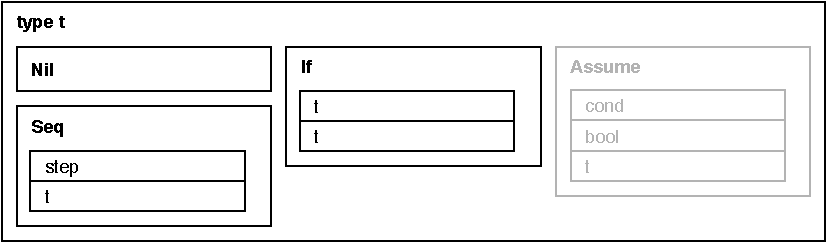
\includegraphics[width=0.9\textwidth]{implementation/figures/node}
    \caption{An illustration of the CFG node types found in EBA.}
    \label{cfg-nodes}
\end{figure}

\noindent Seq-nodes contain a \textit{step} which models a statement in the input source code. When a \textit{Seq}-node is discovered in the tree, the --- possibly multiple --- effects of its containing step are explored. An illustration of this node can be seen in Figure \ref{cfg-step}. These possibly multiple effects raise a problem; since a given step contains a set of effects, the order of these effects are therefore not known and all orders of executing these effects must be explored. This must be done, since a given ordering of effects can lead to a bug, while a different order might not. All permutations of the set of effects must therefore be found and mapped to a given region, while also preserving the information of the other permutations for that given region. Furthermore, the transition function of the monitor automata must be evaluated on the current input, resulting in a new state of that automata which again must also be stored for that region. 

\begin{figure}[H]
    \centering
    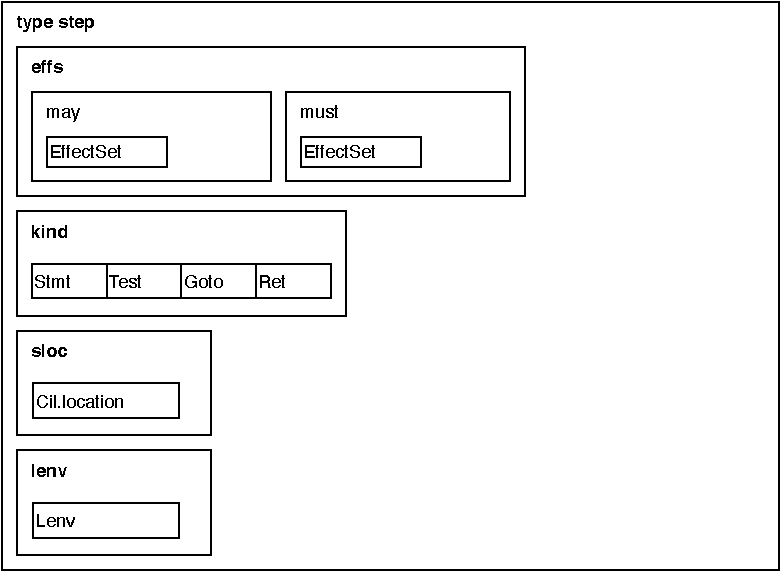
\includegraphics[width=0.9\textwidth]{implementation/figures/step}
    \caption{An illustration of the step type and its containing structures found in EBA.}
    \label{cfg-step}
\end{figure}

\noindent This map can be formalized as the function $m: region \rightarrow { checker\_state }$ where $ checker\_state $ is the internal state of the monitor automata. Using this map it is possible to apply each permutation of effects and fold this list of effects into a modified map with possibly altered automata states for their corresponding regions. The resulting map can be explored in order to find any accepting states of monitor automata for a given region. 

\newpar Given that the map maps a region to the state of monitor automatas, the length of the map will never be larger than the number of regions in the input source file. The size of the set of possible monitor automata states for a given region depends on the effects of a statement operating on a given region. Given a large number of possible effects of a statement the resulting set of permutations of these effects will naturally grow. A set of $N$ effects will result in $N!$ permutations; in other words, the number of monitor automata states for a given region will therefore in the worst case be $|effects|!$. In practice statements lead to a small number of effects and this has not posed a problem during testing.

\newpar When all paths in the CFG tree structure have been explored, the regions which map to accepting states along with their location and traces are extracted from the mapping and presented to the user as possible bugs. 

\newpar This approach can be described in pseudocode as follows.

\begin{algorithm}[H]
\begin{algorithmic}
    \Function{explore\_paths} {$tree\_node$} {$map$} 
        \If {$tree\_node$ is $\mathit{Nil}$}    
            \State{\Return $map$}
        \ElsIf {$tree\_node$ is $\mathit{If}(t, f)$}
            \State{$true\_branch \gets $ \Call{explore\_paths}{t}}
            \State{$false\_branch \gets $ \Call{explore\_paths}{f}} 
            \State{\Return \Call{union}{$true\_branch$, $false\_branch$}}
        \ElsIf {$tree\_node$ is $\mathit{Seq}(step, next)$}
            \State{effects $\gets$ step.effects}
            \If{\Call{is\_empty}{effects}}
                \Return{\Call{explore\_paths}{remaining, map}}
            \EndIf
            \State{permutations $\gets$ \Call{find\_permutations}{effects}}
            \State{\Return \State{\Call{fold}{\Call{fold}{{\Call{apply\_transition}{effect, map}) {map, effects}}}}}}
            
            \Comment{Find all possible states for permutations.}

            \Comment{Add these states to the region map.}
        \EndIf      
    \EndFunction
    \\
    \Function{apply\_transition} {effect, map}
        \State{region $\gets$ effect.region}
        \State{previous\_states\_for\_region $\gets$ \Call{find\_default}{[initial\_state], r, map}}
        \State states $\gets$ \Call{fold}{\Call{transition} {state, effect, previous\_states\_for\_region}}
        \State{\Return {\Call{add}{map, region, states}}}
    \EndFunction
    \\
    \State{tree $\gets $\Call{generate\_tree} {input\_file}}
    \State{map $\gets $ \Call{explore\_paths}{tree}}
\end{algorithmic}
\end{algorithm}

\subsection{Automata Signatures}

The signature of monitor automata must be implemented in order to use the bug checker with EBA. The implementation of a given monitor automata is passed to the aforementioned \texttt{Make} module and is then used to evaluate states based on the effects of regions. The signature of the monitor automata specifies a \texttt{state} as a discriminated union type, describing the possible states of the automata as well as a transition function, \texttt{transition}, which takes a previous state of the monitor along with an input effect. 

\newpar In order to provide the user with detailed error reports this state is encapsulated in a \texttt{checker state} structure which keeps track of the current trace through the CFG along with granular location details for discovered possible bugs. Providing this information requires that the current CFG node must also be passed to the automata, due to the architecture of the EBA framework. The full signature for the transition function is therefore $transition: \mathit{checker\_state} \rightarrow \mathit{effect} \rightarrow \mathit{step} \rightarrow \mathit{checker\_state}$. A concrete example of a $checker\_state$ structure can be seen in Figure \ref{checker-state}.

\begin{figure}[H]
    \centering
    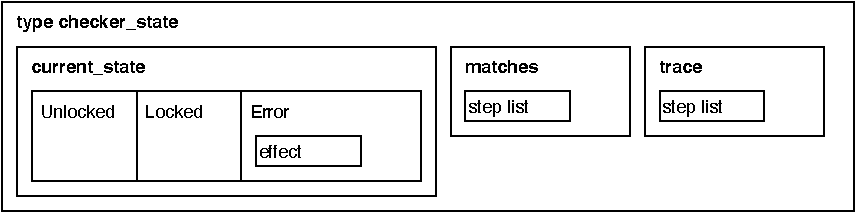
\includegraphics[width=0.9\textwidth]{implementation/figures/checker-state}
    \caption{An illustration of the $checker\_state$ structure for a double-unlock monitor.}
    \label{checker-state}
\end{figure}